% =====================================================================
%  DLE-AI-202 HOMEWORK 1 REPORT, Weeks 1-2, PyTorch  (IEEE two-column)
%  Self-contained: uses only the standard IEEEtran class and standard
%  packages. No .sty files or logos needed.
%  Compile:  tectonic report.tex   (or pdflatex report.tex, twice)
%  Submit the PDF as report.pdf.
% =====================================================================
\documentclass[conference,a4paper]{IEEEtran}
\usepackage{amsmath,amssymb}
\usepackage{graphicx}
\usepackage{booktabs}
\usepackage{xcolor}
\usepackage{url}

% grey placeholder text: delete the \hint{...} and write your answer
\newcommand{\hint}[1]{{\color{gray}\itshape[#1]}}
% graded subsection heading with points on the right
\newcommand{\task}[2]{\subsection{#1\hfill[#2]}}

\begin{document}

\title{DLE-AI-202 Deep Learning, Homework 1:\\
Neural-Network Foundations in PyTorch (Weeks 1--2)}

\author{\IEEEauthorblockN{Alasgarov Teymur}
\IEEEauthorblockA{Student ID: \hint{as on Moodle (this seeds your run)}\\
Section / group: M201\\
Date: 15 November 2026 \quad Hours spent: 11}}

\maketitle

\begin{abstract}
In this report I show my code and results for the basic ideas of deep learning in PyTorch. I wrote tensor operations, stable losses, a manual backpropagation for a two-layer network, and a custom autograd function. I also made MLP networks with different weight initialisations, training loops with warmup-cosine scheduling, and hooks to check the layers.

I used the scikit-learn digits dataset for the experiments. They show two problems of deep networks (vanishing gradients and activations that go to zero). I also compared five optimisers and tested six regularisation methods on data with 25\% wrong labels.

My final model is a 3-layer MLP ($64\to128\to64\to10$) with LayerNorm, dropout ($p=0.15$) and AdamW. It gets a test accuracy of \textbf{97.99\%} (test loss 0.1066), which is higher than the 95\% target.
\end{abstract}

\begin{IEEEkeywords}
backpropagation, initialisation, optimisers, regularisation, PyTorch
\end{IEEEkeywords}

% ---------------------------------------------------------------------
\section{Part A: Written Problems (30 pts)}

\task{A1 Shapes and parameter count}{3}
\textbf{(a) Tensor shapes for batch size $N=128$:}
\begin{itemize}\setlength{\itemsep}{0pt}
  \item Layer 1 ($20\to64$): $W^{(1)} \in \mathbb{R}^{64\times 20}$, $\mathbf{b}^{(1)} \in \mathbb{R}^{64}$, $\mathbf{z}^{(1)} \in \mathbb{R}^{128\times 64}$, $\mathbf{a}^{(1)} \in \mathbb{R}^{128\times 64}$.
  \item Layer 2 ($64\to32$): $W^{(2)} \in \mathbb{R}^{32\times 64}$, $\mathbf{b}^{(2)} \in \mathbb{R}^{32}$, $\mathbf{z}^{(2)} \in \mathbb{R}^{128\times 32}$, $\mathbf{a}^{(2)} \in \mathbb{R}^{128\times 32}$.
  \item Layer 3 ($32\to5$): $W^{(3)} \in \mathbb{R}^{5\times 32}$, $\mathbf{b}^{(3)} \in \mathbb{R}^{5}$, $\mathbf{z}^{(3)} \in \mathbb{R}^{128\times 5}$, $\mathbf{a}^{(3)} \in \mathbb{R}^{128\times 5}$.
\end{itemize}
\textbf{(b) Number of parameters:}
$(20\times 64 + 64) + (64\times 32 + 32) + (32\times 5 + 5) = 1344 + 2080 + 165 = \mathbf{3589}$.\\
\textbf{(c) Multiply-adds for one example:}
$20\times 64 + 64\times 32 + 32\times 5 = 1280 + 2048 + 160 = \mathbf{3488}$ MACs.

\task{A2 Losses come from likelihood}{4}
\textbf{(a) From Gaussian NLL to MSE:}\\
$p(y\mid\hat y) = (2\pi\sigma^2)^{-1/2}\exp(-(y-\hat y)^2/(2\sigma^2))$. We take $-\log$ and get:
$\mathcal{L}_{\text{NLL}} = \frac{1}{2}\log(2\pi\sigma^2) + \frac{1}{2\sigma^2}(y-\hat y)^2$.
Then we sum over $N$ points and remove the constant parts that do not depend on the parameters. After that, $\arg\min_\theta \sum \mathcal{L}_{\text{NLL}} = \arg\min_\theta \frac{1}{N}\sum (y_i-\hat y_i)^2 = \arg\min_\theta \text{MSE}$.\\[2pt]
\textbf{(b) Stable BCE:}\\
We use $\log\hat y = -\log(1+e^{-z})$ and $\log(1-\hat y) = -z-\log(1+e^{-z})$:
$L = -[y\log\hat y + (1-y)\log(1-\hat y)] = z(1-y) + \log(1+e^{-z}) = -zy + [z + \log(1+e^{-z})]$.
Because $z + \log(1+e^{-z}) = \log(1+e^z) = \max(z,0) + \log(1+e^{-|z|})$, we get
$L = \max(z,0) - zy + \log(1+e^{-|z|})$.\\
\emph{Why there is no overflow:} $-|z|$ is never positive, so $e^{-|z|}$ is between 0 and 1. This means $\log(1+e^{-|z|})$ is between 0 and $\ln 2$. We never calculate $e^{z}$ for a big $z$, and we never take $\log(0)$.\\[2pt]
\textbf{(c) Gradient:}\\
$\frac{\partial L}{\partial z} = -y(1-\sigma(z)) + (1-y)\sigma(z) = \sigma(z) - y = \hat y - y$.

\task{A3 Backpropagation by hand}{6}
\textbf{(a) Forward pass:}\\
$\mathbf{z}^{(1)} = W^{(1)}\mathbf{x} + \mathbf{b}^{(1)} = \begin{pmatrix}-1\\1\end{pmatrix}$,
$\mathbf{h} = \operatorname{ReLU}(\mathbf{z}^{(1)}) = \begin{pmatrix}0\\1\end{pmatrix}$,
$\mathbf{z}^{(2)} = W^{(2)}\mathbf{h} + \mathbf{b}^{(2)} = \begin{pmatrix}1\\2\end{pmatrix}$.\\
$\mathbf{p} = \operatorname{softmax}(\mathbf{z}^{(2)}) = \begin{pmatrix}\frac{1}{1+e}\\\frac{e}{1+e}\end{pmatrix} \approx \begin{pmatrix}0.2689\\0.7311\end{pmatrix}$,
$L = -\log p_1 = \log(1+e) \approx \mathbf{1.3133}$.\\[2pt]
\textbf{(b) Layer 2 gradients:}\\
$\boldsymbol\delta^{(2)} = \frac{\partial L}{\partial \mathbf{z}^{(2)}} = \mathbf{p} - \mathbf{y} = \begin{pmatrix}-0.7311\\0.7311\end{pmatrix}$.\\
$\frac{\partial L}{\partial W^{(2)}} = \boldsymbol\delta^{(2)}\mathbf{h}^T = \begin{pmatrix}0 & -0.7311\\0 & 0.7311\end{pmatrix}$, \quad
$\frac{\partial L}{\partial \mathbf{b}^{(2)}} = \boldsymbol\delta^{(2)} = \begin{pmatrix}-0.7311\\0.7311\end{pmatrix}$.\\[2pt]
\textbf{(c) Layer 1 gradients:}\\
$\frac{\partial L}{\partial \mathbf{h}} = (W^{(2)})^T \boldsymbol\delta^{(2)} = \begin{pmatrix}-1.4621\\0.7311\end{pmatrix}$.
Then we multiply by the ReLU gate: $\boldsymbol\delta^{(1)} = \frac{\partial L}{\partial \mathbf{h}} \odot \mathbb{I}(\mathbf{z}^{(1)}>0) = \begin{pmatrix}0\\0.7311\end{pmatrix}$.\\
$\frac{\partial L}{\partial W^{(1)}} = \boldsymbol\delta^{(1)}\mathbf{x}^T = \begin{pmatrix}0 & 0\\0.7311 & 1.4621\end{pmatrix}$, \quad
$\frac{\partial L}{\partial \mathbf{b}^{(1)}} = \boldsymbol\delta^{(1)} = \begin{pmatrix}0\\0.7311\end{pmatrix}$.\\[2pt]
\textbf{(d) Dead ReLU:}
Unit 1 gets zero gradient because $z_1^{(1)} = -1 \le 0$ and $\operatorname{ReLU}'(z)=0$ for $z<0$. If this is true for all training examples, the neuron never changes. This is the dying-ReLU problem, and we lose this neuron forever.

\task{A4 Activations and vanishing gradients}{4}
\textbf{(a) Sigmoid derivative:}\\
$\sigma'(z) = \frac{e^{-z}}{(1+e^{-z})^2} = \sigma(z)(1-\sigma(z))$. Let $u=\sigma(z)\in(0,1)$; $\frac{d}{du}[u(1-u)] = 1-2u=0 \implies u=1/2$ (at $z=0$). So the maximum of $\sigma'(z)$ is $\mathbf{0.25}$.\\[2pt]
\textbf{(b) Number of layers:}\\
$0.25^L < 10^{-6} \iff 4^L > 10^6 \iff L > \frac{6}{\log_{10} 4} \approx 9.966 \implies \mathbf{L \ge 10}$.\\[2pt]
\textbf{(c) Derivatives of Swish and GELU:}\\
• Swish: $f'(z) = \sigma(z) + z\sigma'(z) = \mathbf{\sigma(z) + z\sigma(z)(1-\sigma(z))}$.\\
• GELU: With $\Phi'(z) = \varphi(z)$, $f'(z) = \mathbf{\Phi(z) + z\varphi(z)}$.

\task{A5 Initialisation}{4}
\textbf{(a) He variance:}\\
$\operatorname{Var}(z) = \sum_{j=1}^n \mathbb{E}[w_j^2]\mathbb{E}[a_j^2] = n\operatorname{Var}(w)\mathbb{E}[a^2]$. With ReLU, half of the values become zero, so $\mathbb{E}[a^2] = \frac{1}{2}\operatorname{Var}(z_{\text{prev}})$.
We want $\operatorname{Var}(z)=\operatorname{Var}(z_{\text{prev}})$, so $\frac{n}{2}\operatorname{Var}(w)=1 \implies \mathbf{\operatorname{Var}(w)=2/n}$.\\[2pt]
\textbf{(b) Std for $784\to256$:}\\
$\sigma_{\text{He}} = \sqrt{2/784} \approx \mathbf{0.0505}$; \quad
$\sigma_{\text{Xavier}} = \sqrt{2/(784+256)} = \sqrt{1/520} \approx \mathbf{0.0439}$.\\[2pt]
\textbf{(c) Zero initialisation:}\\
All hidden units give the same activations and get the same gradients $\delta_j a_k$. The symmetry never breaks, so all units learn the same feature.\\[2pt]
\textbf{(d) Initial loss and bugs:}\\
With random initialisation, the predictions are almost equal ($p_k=1/10$), so $L = \ln 10 \approx \mathbf{2.3026}$.
Two bugs can make it bigger: (1) the initial weights are too large ($\sigma=1.0$), so the logits are big and the wrong predictions are very confident; (2) we give softmax probabilities to \texttt{nn.CrossEntropyLoss}, so softmax is applied two times.

\task{A6 Optimisers}{4}
\textbf{(a) SGD vs Momentum ($f'(w)=10w$):}\\
• SGD: $w_1 = 1 - 0.05(10) = \mathbf{0.5}$; $w_2 = 0.5 - 0.05(5) = \mathbf{0.25}$.\\
• Momentum: $v_1 = 0.05(10) = 0.5 \implies w_1 = 1 - 0.5 = \mathbf{0.5}$.
$v_2 = 0.9(0.5) + 0.05(5) = 0.70 \implies w_2 = 0.5 - 0.70 = \mathbf{-0.20}$.\\
\emph{What I see:} Momentum keeps the speed from step 1, so it goes past the minimum ($w^*=0$) to the negative side. SGD goes to the minimum in a smooth way, without crossing it.\\[2pt]
\textbf{(b) First Adam update ($g_1=0.2$):}\\
$m_1 = (1-\beta_1)g_1 = 0.02 \implies \hat m_1 = \frac{0.02}{1-0.9} = 0.2 = g_1$.\\
$v_1 = (1-\beta_2)g_1^2 = 4\times 10^{-5} \implies \hat v_1 = \frac{4\times 10^{-5}}{1-0.999} = 0.04 = g_1^2$.\\
Step: $\Delta w = -\eta \frac{\hat m_1}{\sqrt{\hat v_1}+\epsilon} = -\eta \frac{0.2}{0.2+\epsilon} \approx \mathbf{-\eta}$ (the size of the step is exactly $\eta$).\\[2pt]
\textbf{(c) Decoupled weight decay (AdamW):}\\
In normal Adam, we add $\lambda w$ to the gradient, so the decay is divided by $\sqrt{v_t}$. Because of this, weights that update often get \emph{less} decay than weights that update rarely. AdamW applies $w \leftarrow (1-\eta\lambda)w$ directly, so the decay is the same for all weights.

\task{A7 Regularisation}{3}
\textbf{(a) Weight decay is the same as L2:}\\
For $J(\mathbf{w}) = L(\mathbf{w}) + \frac{\lambda}{2}\|\mathbf{w}\|^2$, $\nabla J = \nabla L + \lambda\mathbf{w}$.
SGD step: $\mathbf{w}_{t+1} = \mathbf{w}_t - \eta(\nabla L + \lambda\mathbf{w}_t) = \mathbf{(1-\eta\lambda)\mathbf{w}_t - \eta\nabla L(\mathbf{w}_t)}$, so the weights are first multiplied by $(1-\eta\lambda)$ and then the gradient step is done.\\[2pt]
\textbf{(b) Expected value of inverted dropout:}\\
Let $m\sim\text{Bernoulli}(1-p)$. $a' = m \frac{a}{1-p}$.
$\mathbb{E}[a'] = \frac{a}{1-p}\mathbb{E}[m] = \frac{a}{1-p}(1-p) = \mathbf{a}$.\\[2pt]
\textbf{(c) BatchNorm in training and in testing:}\\
In training, BatchNorm uses the mean and variance of the current mini-batch ($\mu_{\mathcal{B}}, \sigma_{\mathcal{B}}^2$). This adds some randomness, which works like regularisation. At test time, the output must not depend on the other examples in the batch (even when batch size is 1). So we use the running mean and variance ($\mu_{\text{run}}, \sigma^2_{\text{run}}$) that we saved during training.

\task{A8 Debugging}{2}
\begin{enumerate}\setlength{\itemsep}{1pt}
  \item[(i)] \textbf{Cause:} The gradients are zero or detached (for example, no \texttt{optimizer.step()}, $\eta=0$, or all ReLUs are dead). \textbf{Check:} Print \texttt{p.grad.abs().mean()} for the parameters and see if the gradients exist and are not zero.
  \item[(ii)] \textbf{Cause:} The gradients explode and the numbers overflow, first to $\infty$ and then to \texttt{NaN} (for example, the learning rate is too high or there is no clipping). \textbf{Check:} Turn on gradient clipping (\texttt{clip\_grad\_norm\_}) and make the learning rate $10\times$ smaller.
  \item[(iii)] \textbf{Cause:} Strong overfitting (the model is too big and has too little regularisation). \textbf{Check:} Look at the gap between the train loss and the validation loss. Then add weight decay ($\lambda=10^{-4}$) or dropout.
  \item[(iv)] \textbf{Cause:} The model is still in training mode (\texttt{model.train()}), so Dropout is still on and BatchNorm uses batch statistics. \textbf{Check:} Make sure we call \texttt{model.eval()} before evaluation.
\end{enumerate}

% ---------------------------------------------------------------------
\section{Part B: Code Status}
All the unit tests for the five required modules in \texttt{src/} and for the bonus code pass:
\begin{quote}
\texttt{pytest tests/ -v} $\longrightarrow$ \textbf{36 passed in 1.48s}
\end{quote}
This includes 7/7 tests for tensor basics and losses (B1), 7/7 for manual MLP backpropagation and Swish autograd (B2), 9/9 for the MLP module and initialisers (B3), 7/7 for training and schedulers (B4), 4/4 for hook diagnostics (B5), and 2/2 for custom Adam and MixUp (Bonus).

% ---------------------------------------------------------------------
\section{Part E: Experiments (15 pts)}

\task{E1 Depth and initialisation}{4}
In a 10-layer MLP, the initialisation decides if the signal and the gradients can go through all the layers. With \texttt{sigmoid + xavier}, the gradients vanish very strongly ($\text{grad ratio} = 1.05\times 10^{-6}$). This is close to the theory bound $(0.25)^{10} \approx 9.54\times 10^{-7}$, and the validation accuracy stays at random guessing (0.107).
With \texttt{relu + normal(0.01)}, the activations in the forward pass become smaller and smaller and go to zero ($\sigma^{10} \ll 1$). The network cannot learn useful features (val acc 0.087).
\texttt{relu + xavier} keeps the forward signal, but the gradients get bigger over 10 layers ($\text{grad ratio} = 1.73$), and it reaches 0.867 val acc. At the end, \texttt{relu + he} keeps the variance of the activations about the same in all layers ($\text{grad ratio} = 0.941 \approx 1.0$). It gives the best validation accuracy, \textbf{0.920}.

\task{E2 Optimisers}{3}
I used the same architecture, seed and data with $\eta=0.05$. All five optimisers gave good validation accuracy. RMSprop was the best (0.973), then Adam (0.963), SGD+momentum (0.963), AdamW (0.960) and plain SGD (0.947).
Momentum and adaptive optimisers learned faster at the start because they reduce the zig-zag movement. But one learning rate is not a fair way to compare optimisers. Adaptive methods scale the update by $1/\sqrt{v_t + \epsilon}$, so they work best with small learning rates ($\sim 10^{-3}$). Plain SGD needs bigger steps ($10^{-1}$ to $10^{-2}$) to move on flat parts of the loss surface.

\task{E3 Regularisation}{4}
Table~\ref{tab:reg} shows how regularisation works on 300 digits images with 25\% wrong labels. The baseline memorises the noise fully (train acc 1.000, test 0.809). Dropout ($p=0.5$) stops the features from depending on each other, and the validation loss goes down to 0.601 (test acc 0.837).
BatchNorm is different. Its learnable scale and shift make it easier to memorise the wrong labels, so test accuracy goes down to 0.791. Weight decay punishes large weights, so the logits are less overconfident. The combination (\texttt{dropout+wd+early}) gives the best generalisation (test acc \textbf{0.859}). It stops at epoch 46 when train accuracy is 0.740, which is close to the real share of clean labels ($75\%$).

\begin{table}[!t]
\centering
\caption{Regularisation on 300 images with 25\% wrong labels}
\label{tab:reg}
\setlength{\tabcolsep}{4pt}
\begin{tabular}{@{}lcccc@{}}
\toprule
Configuration & Train acc & Val loss min & Val loss last & Test acc \\
\midrule
Baseline            & 1.000 & 0.739 & 0.910 & 0.809 \\
Dropout (0.5)       & 0.860 & 0.601 & 0.672 & 0.837 \\
Batch norm          & 1.000 & 0.699 & 0.838 & 0.791 \\
Weight decay (0.5)  & 1.000 & 0.723 & 0.756 & 0.807 \\
Early stopping (8)  & 1.000 & 0.750 & 0.763 & 0.791 \\
Combination         & 0.740 & 0.663 & 0.664 & \textbf{0.859} \\
MixUp (0.4) [Bonus] & 0.380 & 0.680 & 0.850 & 0.757 \\
\bottomrule
\end{tabular}
\end{table}

\task{E4 Final model}{4}
I tuned the model only on validation results. The chosen model is a 3-layer MLP ($64\to128\to64\to10$) with ReLU, LayerNorm and Dropout ($p=0.15$). I trained it with AdamW ($\text{lr}=2\times 10^{-3}$, $\text{weight\_decay}=10^{-4}$), a 50-epoch warmup-cosine schedule and gradient clipping ($\text{clip\_norm}=1.0$).
I tested on the test set only one time. The test loss is \textbf{0.1066} and the test accuracy is \textbf{0.9799} ($98.0\% \ge 95\%$, best epoch 34). Fig.~\ref{fig:final} shows that the training was stable and there was no overfitting. Most mistakes were between digits that look similar: $(3 \to 8, 4\times)$, $(4 \to 9, 1\times)$ and $(1 \to 4, 1\times)$.

\begin{figure}[!t]
\centering
\IfFileExists{figures/final_curves.png}{%
  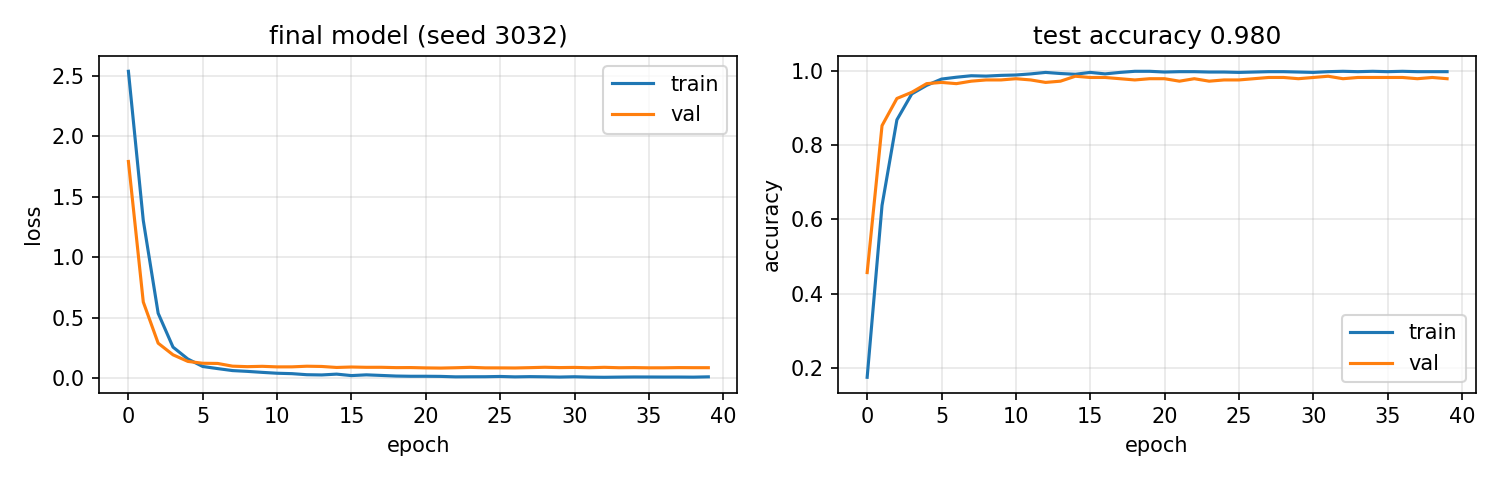
\includegraphics[width=\columnwidth]{figures/final_curves.png}%
}{%
  \fbox{\parbox[c][4cm][c]{0.9\columnwidth}{\centering
  figures/final\_curves.png not found}}%
}
\caption{Training and validation curves of the final model (warm-up + cosine schedule, gradient clipping).}
\label{fig:final}
\end{figure}

% ---------------------------------------------------------------------
\section{Part C: Reflection and Disclosure (10 pts)}

\task{C1 Trace a gradient}{4}
To find the gradient of weight $W^{(1)}_{j,k}$ (from input $j$ to hidden unit $k$), I follow \texttt{manual\_mlp.backward}. First, \texttt{delta2 = (probs - Y) / n} gives $\delta^{(2)}_{i,c} = \frac{1}{n}(p_{i,c} - Y_{i,c}) = \partial L / \partial z^{(2)}_{i,c}$. This joins softmax and mean cross-entropy in one step.
Next, \texttt{delta1 = (delta2 @ W2.T) * act\_derivative(z1, a1, act)} sends the error back to the hidden layer. The activation derivative is multiplied element by element, $f'(z^{(1)}_{i,k})$ ($1 - a_1^2$ for tanh, $\mathbf{1}_{z_1>0}$ for ReLU). It controls how much of the error $\sum_c \delta^{(2)}_{i,c} W^{(2)}_{k,c}$ goes through.
At the end, \texttt{gW1 = X.T @ delta1} computes $\partial L / \partial W^{(1)}_{j,k} = \sum_{i=1}^n X_{i,j} \delta^{(1)}_{i,k}$. It adds up, over the batch, the input $X_{i,j}$ times the error $\delta^{(1)}_{i,k}$ of the hidden unit.

\task{C2 Lines that must not be removed}{3}
Two important lines that we must not remove, because the code breaks without any error, are:
\textbf{(1) \texttt{optimizer.zero\_grad(set\_to\_none=True)}} in \texttt{train\_one\_epoch}. PyTorch adds the new gradients to the old ones every time we call \texttt{backward()}. Without this line, the gradients from all previous batches stay and add up ($\mathbf{g}_t = \sum_{k=1}^t \nabla L_k$). The steps become huge, and the loss goes wrong or becomes NaN, but there is no exception.
\textbf{(2) \texttt{model.eval()}} in \texttt{evaluate}. If the model stays in training mode, \texttt{Dropout} still turns off random activations during evaluation, so the validation metrics are noisy and worse. Also, \texttt{BatchNorm1d} updates its running mean and variance on the validation batches. Then the results are not reproducible, and the evaluation data leaks into the model.

\task{C3 Surprise, and AI-tool disclosure}{3}
One surprising result in E3 was that Batch Normalisation was worse than the baseline without regularisation on test accuracy (0.791 vs 0.809). It also had 1.000 train accuracy and a high final val loss (0.838). The lecture notes say BatchNorm gives a small regularisation effect. But on a small dataset with 25\% label noise, its scale and shift let the model memorise the wrong labels fast, and nothing punishes the weights. When I combined dropout, weight decay and early stopping, the train accuracy stayed lower at 0.740 (close to the 75\% clean data), and the test accuracy was the best, 0.859.
Also, in E1 the gradient ratio of sigmoid+xavier ($1.05\times 10^{-6}$) was very close to the theory bound $0.25^{10}\approx 9.54\times 10^{-7}$ from A4. The network could not learn at all (val acc 0.107).

\textbf{AI-tool disclosure:} I used an AI assistant to check the tensor broadcasting shapes in B1/B2 and to help with the LaTeX template.

% ---------------------------------------------------------------------
\section*{Optional Bonus (up to +10)}
\textbf{MyAdam (+6):} I wrote it in \texttt{src/bonus.py} as a subclass of \texttt{torch.optim.Optimizer}. It keeps moving averages $m_t, v_t$ with bias correction $\hat{m}_t = m_t / (1 - \beta_1^t)$ and $\hat{v}_t = v_t / (1 - \beta_2^t)$. It uses normal $L_2$ weight decay, and the update is $\theta \leftarrow \theta - \frac{\eta}{\sqrt{\hat{v}_t} + \epsilon}\hat{m}_t$. It passes \texttt{tests/test\_bonus.py} and the result is the same as PyTorch's \texttt{torch.optim.Adam} (difference $< 10^{-6}$).

\textbf{MixUp (+4):} I wrote $\tilde{\mathbf{x}} = \lambda \mathbf{x} + (1-\lambda)\mathbf{x}_\pi$ with $\lambda \sim \text{Beta}(\alpha, \alpha)$ in \texttt{bonus.py}. I tested it in the E3 noisy-label setup ($\alpha=0.4$, the row is in Table~\ref{tab:reg}). MixUp stopped the model from memorising the wrong labels, and the train accuracy was only 0.380 (val loss min 0.680, test acc 0.757). But with only 300 images, the strong label mixing made the decision boundaries too soft. I think a smaller $\alpha$ ($\approx 0.1$) would be better.

\section*{Submitted With}
\texttt{src/}, \texttt{hw1\_notebook.ipynb} (with outputs),
\texttt{figures/final\_curves.png}, signed \texttt{pledge.txt}.

\end{document}
